\documentclass[12pt,english]{article}
\usepackage[utf8]{inputenc}
\usepackage[english]{babel}
\usepackage{color}
\usepackage[dvipsnames]{xcolor}
\definecolor{darkblue}{RGB}{0.,0.,139.}
\usepackage{longtable}

\usepackage[top=1in, bottom=1in, left=1in, right=1in]{geometry}

\usepackage{amsmath}
\usepackage{amstext}
\usepackage{amssymb}
\usepackage{setspace}
\usepackage{lipsum}

\usepackage[authoryear]{natbib}
\usepackage{url}
\usepackage{booktabs}
\usepackage[flushleft]{threeparttable}
\usepackage{graphicx}
\usepackage[english]{babel}
\usepackage{pdflscape}
\usepackage[unicode=true,pdfusetitle,
 bookmarks=true,bookmarksnumbered=false,bookmarksopen=false,
 breaklinks=true,pdfborder={0 0 0},backref=false,
 colorlinks,citecolor=black,filecolor=black,
 linkcolor=black,urlcolor=black]
 {hyperref}
\usepackage[all]{hypcap} % Links point to top of image, builds on hyperref
\usepackage{breakurl}    % Allows urls to wrap, including hyperref

\linespread{2}

\begin{document}
\renewcommand{\arraystretch}{0.7}
\setlength\LTleft{0pt}
\setlength\LTright{0pt}

\begin{singlespace}
\title{An Examination of Secondary School Success Indicators}
\end{singlespace}

\author{Luke Denton\thanks{Department of Economics, University of Oklahoma.\
email~address:~\href{mailto:lukedenton@ou.edu}{lukedenton@ou.edu}}}

% \date{\today}
\date{May 10, 2021}

\maketitle

\begin{abstract}
\begin{singlespace}
In this project, I seek to answer a difficult question many experts and organizations have been asking for years: What drives academic performance for students in secondary school? To answer this question, I have computed multiple linear regressions to better understand the impact of different variables on student grade performance. Unsurprisingly, and in accordance with other research, past grades are the strongest indicator, by far, for how well a student does in the present and/or future. This is due to a variety of unobservable variables such as innate ability that underlie academic performance. Despite this, there are strong findings from this analysis: for one, different classes have different aspects that drive student success. This strengthens the idea that is important to focus on student performance at a subject level, not a class-wide level for secondary schooling. 
\end{singlespace}

\end{abstract}
\vfill{}


\pagebreak{}


\section{Introduction}\label{sec:intro}
Education is one of the biggest components of adolescent life. School is where many children spend thousands of hours learning and interacting with teachers, administrators, and their peers. Heralded as a wonderful opportunity to surpass generational poverty, public education provides schooling for millions of students around the world. Despite the widespread existence of public education, a single strategy or set of strategies that help students succeed better in school have largely gone undefined. This drains administrative resources and forces school districts as well as parents to continue to seek the best strategy to foster success for school age children. 

Without a clear strategy for how parents or teachers can best support children in school, children in schools that are poorly funded are susceptible to a lower quality education, and consequently worse life outcomes. The intent of this project is to identify statistically significant, causal factors of student success in secondary school so that these demographics can be furthered studied and their influence in educational performance can be better understood. By identifying specific variables that legitimately affect school performance, resources in schools and at home can be spared from continually exploring new ways to improve student success. Reducing time and capital requirements for educational success will have a profound impact in education systems across the world. In education systems where funding is limited in comparison to other areas, schools and communities will be better equipped to ensure student success. Additionally, in another realm of the world's educational sector, rich economies who spend extreme amounts of money per capita on education will be able to target their spending and eliminate waste of public funds.

\section{Literature Review}\label{sec:litreview}
Much work has been done to better understand the factors that go into student achievement at school. However, there are a multitude of factors at play that shape a student's experience in the classroom. Physical infrastructure in schools, knowledge of language, number of classmates, teacher preparation, teaching methods, access to the internet, travel times, and methods of travel to school are a few of the factors that shape a single student's educational experience. Beginning at the national level with educational standards and guidelines, all the way to a single teacher interacting with students in a classroom, there are many different levels at which education policy is shaped.

Scholars have studied numerous inputs and scenarios to understand what makes a student succeed in their grades. \citet{emotional} Suggests that emotional intelligence, a fairly difficult trait to quantify, serves as a useful indicator of how well students do in university. The study used a questionnaire for first year engineering students in India, and found that higher emotional intelligence scores from the questionnaire also related to increased academic self-efficacy and better performance. \citet{capital} Indicates that higher levels of capital for schools, and even more so for families, yield better educational outcomes. Using the National Longitudinal Survey for Youth, these findings support the unfortunate reality that income inequality yields academic inequality both in school buildings and in homes. \citet{preparation} Takes an alternative approach and attempts to assess student performance from the teacher side of the classroom. Teacher preparation is something that varies from school to school and may be an overlooked indicator for how well students do in school. The study indicates that teacher preparation that is specifically focused on practice yields better teaching outcomes for new teachers after their first year. This is a relieving finding, as opportunities to practice teaching as a student teacher are widely available for aspiring educators. Similarly focusing on teachers, \citet{race} focuses on the effects of racial pairings of students and teachers on school performance. The findings, focused on an experiment in Tennessee, found that there was a positive effect on grades for both black and white students of 3-4 percentage points when paired with a teacher of their same race. This opens up a plethora of questions surrounding racial biases in teachers, however, I will not be addressing the topic of race in this paper.

\section{Data}\label{sec:data}
The primary data source for this research is the student performance database from UCI Machine Learning Data Sets \citet{cortez_silva_2008}. The data tracks secondary school students at two different schools in Portugal. The data measure the first, second, and final period grades of students in mathematics and Portuguese classes, as well as many other demographics concerning home life and school participation. There are 649 total observations in this data set. For an explained list of all the variable codes, see table \ref{tab:descriptions}.

After reading in the CSV files for the math and Portuguese data, my first step in cleaning was to rewrite the 0's in the G3 variable (final grade) as NAs. To deal with the NA's, I decided to use list-wise deletion. Although this is not the most robust manner of dealing with missing data, there did not seem to be any relationship between why a final grade was missing and previous grades. Also, the total number of NA's for math final grades was 38, approximately 9.6 percent of total observations, and only 16 for Portuguese grades, approximately 2.5 percent of the total observations.

After dropping the NA's, I converted many of the variables to factors, as they had been read in as character variables. I also coded in the variable codes for studytime, Fedu, and Medu, as they had been read in as numeric variables. It's important to note that each of my steps in data cleaning were duplicated for both the math and Portuguese data set.

To form a preliminary understanding of the distribution of final grades in both classes, please see figure \ref{fig:fig1} for math and figure \ref{fig:fig2} for Portuguese. The distribution of grades for Portuguese is heavier at the right end, although both distributions are well dispersed across the grading scale. It's important to note that the grading scale used in this data is from 0-20. I will make references to the 100-point scale used in America when discussing research findings.

\section{Empirical Methods}\label{sec:methods}
The main tactic I have used to better understand these indicators is a multiple linear regression model. The basic equation for the multiple linear regression is shown as follows: 
\begin{equation}
        Y = \beta{X} + u
\end{equation} 
In this analysis, the dependent variable (Y) that I am choosing to focus on is G3, a student's final grade recorded in their class. The independent variables (X's) vary depending on the model, but are included to help provide an explanation for the variation in final grades (Y) among students.

\begin{itemize}

\item Model 1: Linear Regression Model
\label{eq:1}
In this model, I included studytime as the sole regressor to see how much of an effect it has on final grades. 
\begin{equation}
    final = \beta_0 + \beta_1studytime + u
\end{equation}

\item Model 2: Multiple Linear Regression Model

This initial model attempts to explain variation in final grades in math based off of what research indicates is a predictor of final grades: midterm grades. I have included the first and second period grades as the only variables in this model to see how much of the variation in the final grade they account for.
\begin{equation}
    final = \beta_0 + \beta_1G1 + \beta_2G2 + u
\end{equation}

\item Model 3: Expanded Multiple Linear Regression Model

This model contains the previous independent variables but also includes new ones in hopes of increasing the amount of variation explained.
\begin{equation}
\begin{split}
    final = & \beta_0 + \beta_1G1 + \beta_2G2 + \beta_3Medu + \beta_4Fedu + \beta_5studytime \\ + & \beta_6address + \beta_7famsize + \beta_8Pstatus + \beta_9activities + u
\end{split}
\end{equation}

\item Model 4: Multiple Linear Regression with all variables

This model was meant to identify variables with a statistically significant p-value, so that they could be further examined in model 5. Please see table \ref{tab:descriptions} for the description of all of the variable codes. 
% sorry dr ransom, I'm not trying to take up extra room in the paper with my equation
\begin{equation}
    \begin{split}
        final = & \beta_0 + \beta_1school + \beta_2sex + \beta3_age + \beta_4address + \beta_5famsize + \beta_6Pstatus \\ + &\beta_7Medu + \beta_8Fedu + \beta_9Mjob + \beta_{10}Fjob + \beta_{11}reason + \beta_{12}guardian \\ + &\beta_{13}traveltime + \beta_{14}studytime + \beta_{15}failures + \beta_{16}schoolsup + \beta_{17}famsup \\ + &\beta_{18}paid + \beta_{19}activities + \beta_{20}nursery + \beta_{21}higher + \beta_{22}internet + \beta_{23}romantic \\ + &\beta_{24}famrel + \beta_{25}freetime + \beta_{26}goout + \beta_{27}Dalc + \beta_{28}Walc + \beta_{29}health \\ + &\beta_{30}absences + \beta_{31}G1 + \beta_{32}G2 + u
    \end{split}
\end{equation}

\item Model 5: MLR With Only Significant Variables
\label{model:5}
This model was computed after regressing every included variable against the final grade in math and Portuguese classes. Different variables were significant for the two classes, but the nature of the models' origin is the same. 
\begin{equation}
\begin{split}
(math) final = & \beta_0 + \beta_1G1 + \beta2_G2 + \beta_3absences + \beta_4health + \beta_5goout \\ & + \beta_6famrel + \beta_7paid + u \\
(port) final = & \beta_0 + \beta_1G1 + \beta2_G2 + \beta_3higher + \beta_4failures + \beta_5traveltime \\& + \beta_6Fjob + \beta_7Mjob + \beta_8age + u
\end{split}
\end{equation}


\end{itemize}


\section{Research Findings}\label{sec:results}
The results for models 1 and 2 for both math and Portuguese grades can be reviewed in table \ref{tab:comparison}. From the first model, we learn that studytime only has a statistically significant effect on math grades for the 'between 5-10' hour category. This phenomenon is supported by many other researchers' findings that suggest that amount spent studying may not help a student obtain a better grade. Oddly enough, though, studytime for Portuguese had a statistically significant effect on final grades across all levels of the variable, and the effect was relatively impactful. It's important to keep in mind that the final grades in this data set are on a scale of 20 points; so, an increase of 1.957 points as a result of studying 5-10 hours per week would be the equivalent of raising your grade by a whole letter grade in the American grading system. This drastic difference in the benefits to time spent studying is also visualized in figures \ref{fig:fig3} and \ref{fig:fig4}. In figure \ref{fig:fig3}, you can see that there is a substantial amount of dispersion among final grades in math within the different categories of time spent studying. Final grades for students who studied more than ten hours ranged from 7 to 20, an American-scale equivalence of 35-100. Across the different categories, there is a very slight positive relationship between increased studytime, but it is not significant. Contrarily, figure \ref{fig:fig4} displays a much more significant positive relationship between studytime and final grades in Portuguese. There is less dispersion among each category, which helps visualize why the coefficients for Model 1 with Portuguese were statistically significant.  

The second model illustrates a commonly known phenomenon in the study of academic performance: the best indicator of a student's future grade is their past grades. First and second period grades for math and Portuguese have statistically significant coefficients of substantial impact. In fact, second period grades for both courses constitute a close to 1:1 relationship with the final grade. Additionally, the R-squared values for model 2 illustrate the significant portion of variation in final grades that are explained by past grades. With a value of 0.935 for math and 0.881 for Portuguese, the unfortunate truth is that it is very difficult to find any other significant contributing factor to final grades besides past grades.

Model 3, composed of different variables that might conceivably affect students' final grades, displays a lack of statistical significance across the board for every single variable that was not included in models 1 or 2. Table \ref{tab:comparison3} illustrates that there simply isn't a strong enough relationship between any of these variables across all students to constitute a causal effect. Also, if the lack of significance was not enough, model 3 improved the R-squared by a whopping 0.001 and 0.002 for math and Portuguese, respectively. 

Model 4 produces different statistically significant coefficients for math and Portuguese. If interested, you can view the full results in tables \ref{tab:6} and \ref{tab:7}. However, since I included only the significant variables in model 5, those tables would be more convenient to reference. See tables \ref{tab:model5m} and \ref{tab:model5p}. For math, the only variable that had a coefficient in the tenths place was famrel, which is a likert scale rating from 1-5 of family relationships. Therefore, the best family relationships distinguished a student's final grade by 0.79, or 3.95 points on an American scale. This is a moderately interesting finding, and could feasibly make the difference in letter grades for a student. Funnily, paying to go to school yielded worse final grade outcomes than students who did not pay to go to school. For Portuguese, there were more significant variables from model 4, but a few did not remain significant in the more specified model 5. Interestingly, all father occupations yielded worse final grades compared to the comparison dummy: staying at home. Also, pursuing higher education yielded better grades, as did failing less classes and an increased travel time to school.

\section{Conclusion}\label{sec:conclusion}
The arduous and seemingly mystical task of understanding what precisely causes a student's performance in school is a subject of careful study and mixed reviews. In an environment where factors from home, school, teachers, and peers all interact, predicting education performance as well as finding causal relationships between indicators is difficult. One major takeaway from this analysis is that classes in different styles can have different causal influences. In our case, math performance was statistically unaffected by age, whereas Portuguese grades had a small but noticeable positive relationship to student age. This was the case for several other variables as well, including the desire to pursue higher education, and father's occupation. One unfortunate takeaway is that time spent studying is not necessarily tied to performing better in classes, more so for math. This absence of causality is an indicator that there are more intangible and difficult to measure variables that are at play. Innate ability, motivation, and attention are all characteristics that academic literature suggest underlie part of these intangible effects. After all, a nearly one-to-one relationship between second term grades and final grades is indicative that there is much more to be learned about why students do well in school in the first place. Perhaps with continued study, different factors of student success will be better understood, so that education systems can more effectively teach students and prepare them for the future.

\vfill
\pagebreak{}
\begin{spacing}{1.0}
\bibliographystyle{jpe}
\nocite{*}
\bibliography{PS11_Denton.bib}
\addcontentsline{toc}{section}{References}
\end{spacing}

\vfill
\pagebreak{}
\clearpage

%========================================
% FIGURES AND TABLES 
%========================================
\section{Figures and Tables}
%----------------------------------------
% Figure 1
%----------------------------------------
\begin{figure}[ht]
\centering
\bigskip{}
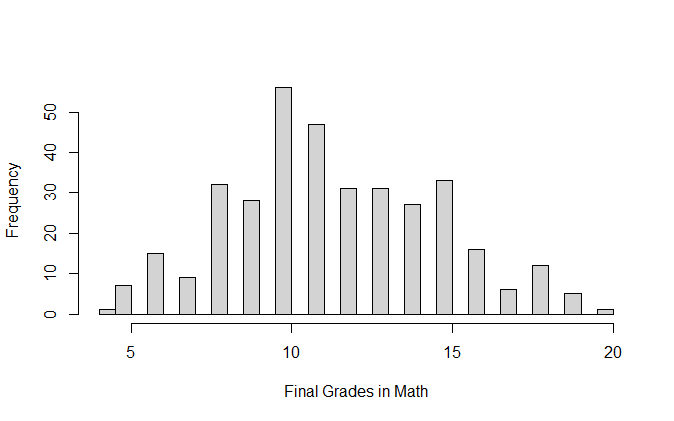
\includegraphics[width=.95\linewidth]{hist_mathgrades.png}
\caption{Distribution of Final Grades in Math}
\label{fig:fig1}
\end{figure}
%----------------------------------------
% Figure 2
%----------------------------------------
\begin{figure}[ht]
\centering
\bigskip{}
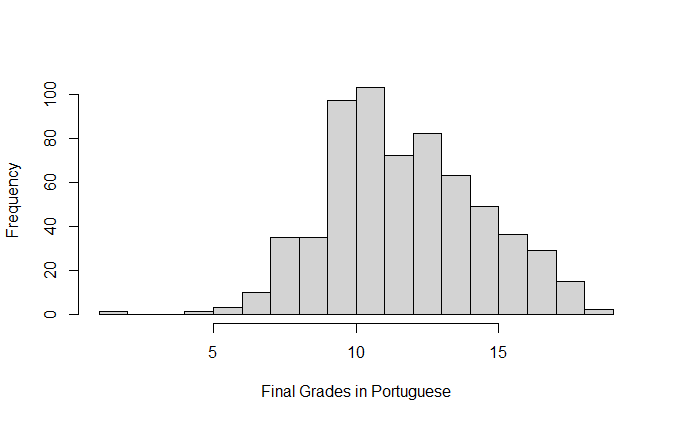
\includegraphics[width=.95\linewidth]{hist_portgrades.png}
\caption{Distribution of Final Grades in Portuguese}
\label{fig:fig2}
\end{figure}
%----------------------------------------
% Figure 3
%----------------------------------------
\begin{figure}[ht]
\centering
\bigskip{}
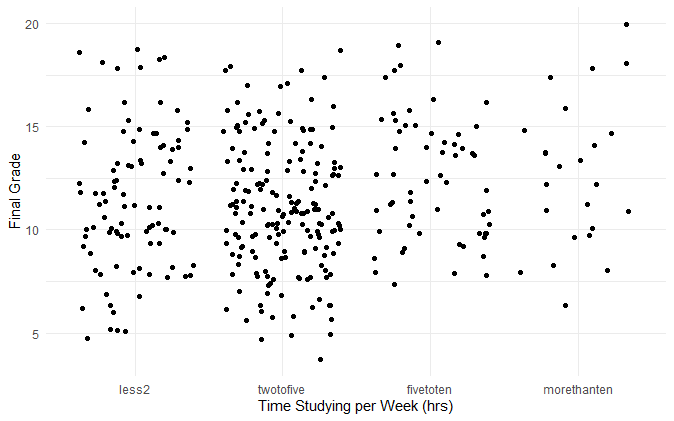
\includegraphics[width=.95\linewidth]{math_grades.png}
\caption{Relationship between studying and math final grade}
\label{fig:fig3}
\end{figure}
%----------------------------------------
% Figure 4
%----------------------------------------
\begin{figure}[ht]
\centering
\bigskip{}
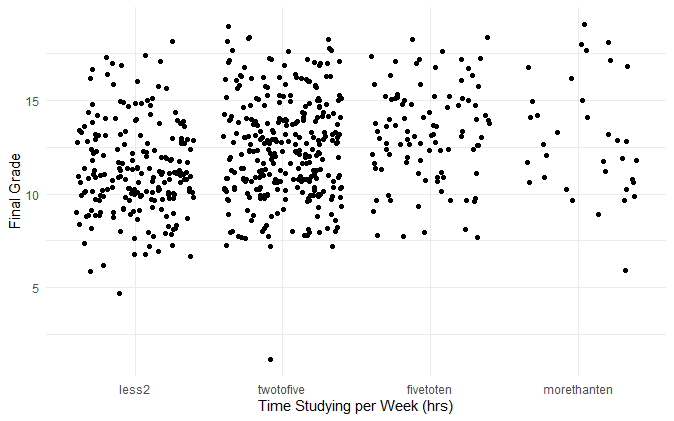
\includegraphics[width=.95\linewidth]{port_grades.png}
\caption{Relationship between studying and Portuguese final grade}
\label{fig:fig4}
\end{figure}
\pagebreak

%----------------------------------------
% Table 1
%----------------------------------------
\begin{table}[ht]
\caption{Variable Codes and Descriptions}
\label{tab:descriptions} 
\begin{center}
 \begin{tabular}{|c|c|} 
 \hline
 variable & description  \\ [0.5ex] 
 \hline\hline
 school & student's school \\ 
 \hline 
 sex & student's sex \\
 \hline 
age & student's age \\
\hline  
address & student's home address type\\
 \hline 
 famsize & family size \\
 \hline 
 Pstatus & parent's cohabitation status \\
\hline  
Medu & mother's education \\
\hline  
Fedu & father's education\\
 \hline 
 Mjob & mother's job \\
 \hline 
 Fjob & father's job \\
\hline 
reason & reason to choose this school\\
\hline 
guardian & student's guardian\\
\hline 
traveltime & home to school travel time\\
\hline 
studytime & weekly study time (hrs)\\
\hline 
failures & number of past class failures\\
\hline 
schoolsup & extra educational support \\
\hline 
famsup & family educational support \\
\hline 
paid & extra paid classes \\
\hline 
activities & extra-curricular activities \\
\hline 
nursery & attended nursery school\\
\hline 
higher & wants to take higher education \\
\hline 
 internet & Internet access at home \\
 \hline 
romantic & with a romantic relationship \\
\hline 
famrel & quality of family relationships \\
\hline 
freetime & free time after school\\ 
\hline 
goout & going out with friends \\
\hline 
Dalc & workday alcohol consumption  \\
\hline
Walc & weekend alcohol consumption\\
\hline 
health & current health status \\
\hline 
absences & number of school absences\\
\hline 
final & final grade\\
\hline
\end{tabular}
\end{center}
\end{table}
\pagebreak

%----------------------------------------
% Table 2
%----------------------------------------
\begin{table}
\centering
\caption{Models 1 and 2 compared between math and Portuguese, respectively}
\label{tab:comparison}
\begin{tabular}[t]{lcccc}
\toprule
  & Model 1 (math) & Model 1 (Port) & Model 2 (math) & Model 2 (Port)\\
\midrule
(Intercept) & 11.467*** & 11.270*** & 0.195 & 0.738***\\
 & (0.332) & (0.182) & (0.166) & (0.172)\\
studytimetwotofive & -0.401 & 1.111*** &  & \\
 & (0.407) & (0.237) &  & \\
studytimefivetoten & 1.092** & 1.957*** &  & \\
 & (0.531) & (0.321) &  & \\
studytimemorethanten & 1.199 & 1.788*** &  & \\
 & (0.730) & (0.477) &  & \\
G1 &  &  & 0.112*** & 0.216***\\
 &  &  & (0.031) & (0.031)\\
G2 &  &  & 0.887*** & 0.763***\\
 &  &  & (0.032) & (0.031)\\
\midrule
Num.Obs. & 357 & 633 & 357 & 633\\
R2 & 0.036 & 0.069 & 0.935 & 0.881\\
R2 Adj. & 0.028 & 0.064 & 0.934 & 0.881\\
AIC & 1845.7 & 3014.9 & 882.7 & 1709.7\\
BIC & 1865.1 & 3037.1 & 898.2 & 1727.5\\
Log.Lik. & -917.872 & -1502.434 & -437.327 & -850.852\\
F & 4.378 & 15.423 & 2533.295 & 2334.862\\
\bottomrule
\multicolumn{5}{l}{\textsuperscript{} * p $<$ 0.1, ** p $<$ 0.05, *** p $<$ 0.01}\\
\end{tabular}
\end{table}
%----------------------------------------
% Table 3
%----------------------------------------
\begin{table}
\caption{Model 3 compared between math and Portuguese, respectively}
\label{tab:comparison3}
\centering
\begin{tabular}[t]{lcc}
\toprule
  & Model 3 (math) & Model 3 (Port)\\
\midrule
(Intercept) & 0.245 & 1.049**\\
 & (0.831) & (0.530)\\
G1 & 0.113*** & 0.210***\\
 & (0.032) & (0.032)\\
G2 & 0.885*** & 0.760***\\
 & (0.034) & (0.032)\\
Meduprmry & -0.148 & -0.143\\
 & (0.505) & (0.395)\\
Medumdlschl & -0.179 & -0.039\\
 & (0.496) & (0.395)\\
Meduscndry & -0.253 & -0.122\\
 & (0.499) & (0.400)\\
Meducollege & -0.116 & 0.043\\
 & (0.502) & (0.403)\\
Feduprmry & 0.309 & -0.149\\
 & (0.613) & (0.369)\\
Fedumdlschl & 0.143 & -0.145\\
 & (0.613) & (0.371)\\
Feduscndry & 0.140 & -0.233\\
 & (0.612) & (0.378)\\
Feducollege & 0.094 & -0.289\\
 & (0.615) & (0.382)\\
studytimetwotofive & -0.023 & 0.189**\\
 & (0.109) & (0.087)\\
studytimefivetoten & 0.057 & 0.179\\
 & (0.143) & (0.119)\\
studytimemorethanten & 0.112 & 0.038\\
 & (0.197) & (0.176)\\
addressU & 0.149 & -0.011\\
 & (0.112) & (0.085)\\
famsizeLE3 & -0.063 & -0.026\\
 & (0.101) & (0.085)\\
PstatusT & -0.140 & -0.063\\
 & (0.149) & (0.120)\\
activitiesyes & -0.019 & -0.019\\
 & (0.092) & (0.076)\\
\midrule
Num.Obs. & 357 & 633\\
R2 & 0.936 & 0.883\\
R2 Adj. & 0.933 & 0.880\\
AIC & 905.4 & 1730.3\\
BIC & 979.1 & 1814.8\\
Log.Lik. & -433.697 & -846.130\\
F & 291.678 & 272.724\\
\bottomrule
\multicolumn{3}{l}{\textsuperscript{} * p $<$ 0.1, ** p $<$ 0.05, *** p $<$ 0.01}\\
\end{tabular}
\end{table}
%----------------------------------------
% Table 4
%----------------------------------------
\begin{table}
\caption{Model 5, Math(using only signif. vars from Model 4)}
\label{tab:model5m}
\centering
\begin{tabular}[t]{lc}
\toprule
  & Model 1\\
\midrule
(Intercept) & 0.320\\
 & (0.317)\\
G1 & 0.111***\\
 & \vphantom{1} (0.031)\\
G2 & 0.876***\\
 & (0.032)\\
absences & -0.011*\\
 & (0.005)\\
health & -0.067**\\
 & (0.031)\\
goout & -0.082**\\
 & (0.040)\\
famrel & 0.158***\\
 & (0.049)\\
paidyes & -0.124\\
 & (0.086)\\
\midrule
Num.Obs. & 357\\
R2 & 0.939\\
R2 Adj. & 0.938\\
AIC & 868.8\\
BIC & 903.7\\
Log.Lik. & -425.394\\
F & 766.354\\
\bottomrule
\multicolumn{2}{l}{\textsuperscript{} * p $<$ 0.1, ** p $<$ 0.05,}\\
\multicolumn{2}{l}{*** p $<$ 0.01}\\
\end{tabular}
\end{table}
%----------------------------------------
% Table 5
%----------------------------------------
\begin{table}
\caption{Model 5, Portuguese (using only signif. vars from Model 4)}
\label{tab:model5p}
\centering
\begin{tabular}[t]{lc}
\toprule
  & Model 1\\
\midrule
(Intercept) & -1.228**\\
 & (0.612)\\
G1 & 0.222***\\
 & (0.032)\\
G2 & 0.733***\\
 & (0.031)\\
higheryes & 0.257*\\
 & (0.134)\\
failures & -0.222***\\
 & (0.072)\\
traveltime & 0.109**\\
 & (0.050)\\
Fjobhealth & -0.448*\\
 & (0.247)\\
Fjobother & -0.318**\\
 & (0.153)\\
Fjobservices & -0.394**\\
 & (0.161)\\
Fjobteacher & -0.399*\\
 & (0.223)\\
Mjobhealth & 0.227\\
 & (0.164)\\
Mjobother & 0.098\\
 & (0.101)\\
Mjobservices & 0.126\\
 & (0.117)\\
Mjobteacher & 0.309**\\
 & (0.146)\\
age & 0.125***\\
 & (0.033)\\
\midrule
Num.Obs. & 633\\
R2 & 0.888\\
R2 Adj. & 0.885\\
AIC & 1697.9\\
BIC & 1769.2\\
Log.Lik. & -832.974\\
F & 348.778\\
\bottomrule
\multicolumn{2}{l}{\textsuperscript{} * p $<$ 0.1, ** p $<$ 0.05,}\\
\multicolumn{2}{l}{*** p $<$ 0.01}\\
\end{tabular}
\end{table}
%----------------------------------------
% Table 6
%----------------------------------------
\clearpage
\begin{longtable}[c]{lccccc}
\caption{All model results for Math grades} \label{tab:6} \\
\hline 
 & Model 1 & Model 2 & Model 3 & Model 4 & Model 5\\
\endfirsthead
\multicolumn{5}{4}{{\bfseries \tablename\ \thetable{} -- All model results for Math grades}} \\
\hline 
  & Model 1 & Model 2 & Model 3 & Model 4 & Model 5\\
\endhead
\hline {{Continued on next page}} \\ \hline
\endfoot
\hline \hline
\endlastfoot
(Intercept) & 11.467*** & 0.195 & 0.245 & -0.278 & 0.320\\
 & (0.332) & (0.166) & (0.831) & (1.259) & (0.317)\\
studytimetwotofive & -0.401 &  & -0.023 & -0.027 & \\
 & (0.407) &  & (0.109) & (0.119) & \\
studytimefivetoten & 1.092** &  & 0.057 & 0.040 & \\
 & (0.531) &  & (0.143) & (0.163) & \\
studytimemorethanten & 1.199 &  & 0.112 & 0.142 & \\
 & (0.730) &  & (0.197) & (0.216) & \\
G1 &  & 0.112*** & 0.113*** & 0.100*** & 0.111***\\
 &  & (0.031) & (0.032) & (0.035) & (0.031)\\
G2 &  & 0.887*** & 0.885*** & 0.881*** & 0.876***\\
 &  & (0.032) & (0.034) & (0.036) & (0.032)\\
Meduprmry &  &  & -0.148 & -0.185 & \\
 &  &  & (0.505) & (0.518) & \\
Medumdlschl &  &  & -0.179 & -0.192 & \\
 &  &  & (0.496) & (0.517) & \\
Meduscndry &  &  & -0.253 & -0.334 & \\
 &  &  & (0.499) & (0.524) & \\
Meducollege &  &  & -0.116 & -0.297 & \\
 &  &  & (0.502) & (0.539) & \\
Feduprmry &  &  & 0.309 & 0.338 & \\
 &  &  & (0.613) & (0.623) & \\
Fedumdlschl &  &  & 0.143 & 0.231 & \\
 &  &  & (0.613) & (0.624) & \\
Feduscndry &  &  & 0.140 & 0.228 & \\
 &  &  & (0.612) & (0.625) & \\
Feducollege &  &  & 0.094 & 0.226 & \\
 &  &  & (0.615) & (0.636) & \\
addressU &  &  & 0.149 & 0.161 & \\
 &  &  & (0.112) & (0.126) & \\
famsizeLE3 &  &  & -0.063 & -0.079 & \\
 &  &  & (0.101) & (0.105) & \\
PstatusT &  &  & -0.140 & -0.216 & \\
 &  &  & (0.149) & (0.153) & \\
activitiesyes &  &  & -0.019 & -0.014 & \\
 &  &  & (0.092) & (0.097) & \\
schoolMS &  &  &  & -0.109 & \\
 &  &  &  & (0.170) & \\
sexM &  &  &  & -0.039 & \\
 &  &  &  & (0.109) & \\
age &  &  &  & 0.039 & \\
 &  &  &  & (0.048) & \\
Mjobhealth &  &  &  & 0.249 & \\
 &  &  &  & (0.241) & \\
Mjobother &  &  &  & -0.170 & \\
 &  &  &  & (0.159) & \\
Mjobservices &  &  &  & 0.068 & \\
 &  &  &  & (0.177) & \\
Mjobteacher &  &  &  & 0.227 & \\
 &  &  &  & (0.227) & \\
Fjobhealth &  &  &  & 0.229 & \\
 &  &  &  & (0.307) & \\
Fjobother &  &  &  & 0.284 & \\
 &  &  &  & (0.226) & \\
Fjobservices &  &  &  & 0.173 & \\
 &  &  &  & (0.234) & \\
Fjobteacher &  &  &  & 0.240 & \\
 &  &  &  & (0.290) & \\
reasonhome &  &  &  & 0.191 & \\
 &  &  &  & (0.121) & \\
reasonother &  &  &  & 0.011 & \\
 &  &  &  & (0.171) & \\
reasonreputation &  &  &  & 0.079 & \\
 &  &  &  & (0.124) & \\
guardianmother &  &  &  & -0.013 & \\
 &  &  &  & (0.116) & \\
guardianother &  &  &  & -0.349 & \\
 &  &  &  & (0.223) & \\
traveltime &  &  &  & 0.046 & \\
 &  &  &  & (0.073) & \\
failures &  &  &  & 0.033 & \\
 &  &  &  & (0.083) & \\
schoolsupyes &  &  &  & -0.160 & \\
 &  &  &  & (0.144) & \\
famsupyes &  &  &  & 0.104 & \\
 &  &  &  & (0.103) & \\
paidyes &  &  &  & -0.206** & -0.124\\
 &  &  &  & (0.100) & (0.086)\\
nurseryyes &  &  &  & -0.168 & \\
 &  &  &  & (0.120) & \\
higheryes &  &  &  & -0.029 & \\
 &  &  &  & (0.260) & \\
internetyes &  &  &  & -0.002 & \\
 &  &  &  & (0.134) & \\
romanticyes &  &  &  & 0.020 & \\
 &  &  &  & (0.104) & \\
famrel &  &  &  & 0.177*** & 0.158***\\
 &  &  &  & (0.053) & (0.049)\\
freetime &  &  &  & -0.015 & \\
 &  &  &  & (0.051) & \\
goout &  &  &  & -0.093* & -0.082**\\
 &  &  &  & (0.050) & (0.040)\\
Dalc &  &  &  & 0.028 & \\
 &  &  &  & (0.069) & \\
Walc &  &  &  & -0.003 & \\
 &  &  &  & (0.054) & \\
health &  &  &  & -0.085** & -0.067**\\
 &  &  &  & (0.035) & (0.031)\\
absences &  &  &  & -0.011* & -0.011*\\
 &  &  &  & (0.006) & (0.005)\\
\hline
Num.Obs. & 357 & 357 & 357 & 357 & 357\\
R2 & 0.036 & 0.935 & 0.936 & 0.944 & 0.939\\
R2 Adj. & 0.028 & 0.934 & 0.933 & 0.935 & 0.938\\
AIC & 1845.7 & 882.7 & 905.4 & 923.0 & 868.8\\
BIC & 1865.1 & 898.2 & 979.1 & 1120.7 & 903.7\\
Log.Lik. & -917.872 & -437.327 & -433.697 & -410.487 & -425.394\\
F & 4.378 & 2533.295 & 291.678 & 105.238 & 766.354\\
\hline
\multicolumn{5}{2}{\textsuperscript{} * p $<$ 0.1, ** p $<$ 0.05, *** p $<$ 0.01}\\
\end{longtable}
%----------------------------------------
% Table 7
%----------------------------------------
\clearpage
\begin{longtable}[c]{lccccc}
\caption{All model results for Portuguese grades} \label{tab:7} \\
\hline 
 & Model 1 & Model 2 & Model 3 & Model 4 & Model 5\\
\endfirsthead
\multicolumn{5}{4}{{\bfseries \tablename\ \thetable{} -- All model results for Portuguese grades}} \\
\hline 
  & Model 1 & Model 2 & Model 3 & Model 4 & Model 5\\
\endhead
\hline {{Continued on next page}} \\ \hline
\endfoot
\hline \hline
\endlastfoot
(Intercept) & 11.270*** & 0.738*** & 1.049** & -0.346 & -1.228**\\
 & (0.182) & (0.172) & (0.530) & (0.875) & (0.612)\\
studytimetwotofive & 1.111*** &  & 0.189** & 0.103 & \\
 & (0.237) &  & (0.087) & (0.092) & \\
studytimefivetoten & 1.957*** &  & 0.179 & 0.032 & \\
 & (0.321) &  & (0.119) & (0.126) & \\
studytimemorethanten & 1.788*** &  & 0.038 & 0.001 & \\
 & (0.477) &  & (0.176) & (0.182) & \\
G1 &  & 0.216*** & 0.210*** & 0.211*** & 0.222***\\
 &  & (0.031) & (0.032) & (0.033) & (0.032)\\
G2 &  & 0.763*** & 0.760*** & 0.719*** & 0.733***\\
 &  & (0.031) & (0.032) & (0.033) & (0.031)\\
Meduprmry &  &  & -0.143 & 0.010 & \\
 &  &  & (0.395) & (0.398) & \\
Medumdlschl &  &  & -0.039 & 0.054 & \\
 &  &  & (0.395) & (0.402) & \\
Meduscndry &  &  & -0.122 & -0.007 & \\
 &  &  & (0.400) & (0.407) & \\
Meducollege &  &  & 0.043 & 0.065 & \\
 &  &  & (0.403) & (0.422) & \\
Feduprmry &  &  & -0.149 & -0.016 & \\
 &  &  & (0.369) & (0.373) & \\
Fedumdlschl &  &  & -0.145 & 0.055 & \\
 &  &  & (0.371) & (0.378) & \\
Feduscndry &  &  & -0.233 & -0.070 & \\
 &  &  & (0.378) & (0.385) & \\
Feducollege &  &  & -0.289 & -0.052 & \\
 &  &  & (0.382) & (0.395) & \\
addressU &  &  & -0.011 & -0.012 & \\
 &  &  & (0.085) & (0.092) & \\
famsizeLE3 &  &  & -0.026 & -0.052 & \\
 &  &  & (0.085) & (0.086) & \\
PstatusT &  &  & -0.063 & -0.081 & \\
 &  &  & (0.120) & (0.123) & \\
activitiesyes &  &  & -0.019 & 0.042 & \\
 &  &  & (0.076) & (0.079) & \\
schoolMS &  &  &  & -0.075 & \\
 &  &  &  & (0.096) & \\
sexM &  &  &  & -0.118 & \\
 &  &  &  & (0.089) & \\
age &  &  &  & 0.123*** & 0.125***\\
 &  &  &  & (0.037) & (0.033)\\
Mjobhealth &  &  &  & 0.200 & 0.227\\
 &  &  &  & (0.191) & (0.164)\\
Mjobother &  &  &  & 0.093 & 0.098\\
 &  &  &  & (0.107) & (0.101)\\
Mjobservices &  &  &  & 0.168 & 0.126\\
 &  &  &  & (0.131) & (0.117)\\
Mjobteacher &  &  &  & 0.313* & 0.309**\\
 &  &  &  & (0.184) & (0.146)\\
Fjobhealth &  &  &  & -0.350 & -0.448*\\
 &  &  &  & (0.265) & (0.247)\\
Fjobother &  &  &  & -0.350** & -0.318**\\
 &  &  &  & (0.161) & (0.153)\\
Fjobservices &  &  &  & -0.420** & -0.394**\\
 &  &  &  & (0.170) & (0.161)\\
Fjobteacher &  &  &  & -0.361 & -0.399*\\
 &  &  &  & (0.246) & (0.223)\\
reasonhome &  &  &  & 0.086 & \\
 &  &  &  & (0.100) & \\
reasonother &  &  &  & -0.089 & \\
 &  &  &  & (0.131) \vphantom{1} & \\
reasonreputation &  &  &  & -0.011 & \\
 &  &  &  & (0.104) & \\
guardianmother &  &  &  & -0.018 & \\
 &  &  &  & (0.093) & \\
guardianother &  &  &  & 0.094 & \\
 &  &  &  & (0.187) & \\
traveltime &  &  &  & 0.139** & 0.109**\\
 &  &  &  & (0.056) & (0.050)\\
failures &  &  &  & -0.206*** & -0.222***\\
 &  &  &  & (0.075) & (0.072)\\
schoolsupyes &  &  &  & -0.175 & \\
 &  &  &  & (0.131) & \\
famsupyes &  &  &  & -0.014 & \\
 &  &  &  & (0.080) & \\
paidyes &  &  &  & -0.160 & \\
 &  &  &  & (0.162) & \\
nurseryyes &  &  &  & -0.057 & \\
 &  &  &  & (0.095) & \\
higheryes &  &  &  & 0.236* & 0.257*\\
 &  &  &  & (0.140) & (0.134)\\
internetyes &  &  &  & 0.136 & \\
 &  &  &  & (0.098) & \\
romanticyes &  &  &  & -0.022 & \\
 &  &  &  & (0.081) & \\
famrel &  &  &  & 0.010 & \\
 &  &  &  & (0.041) & \\
freetime &  &  &  & -0.031 & \\
 &  &  &  & (0.039) & \\
goout &  &  &  & -0.058 & \\
 &  &  &  & (0.038) & \\
Dalc &  &  &  & -0.075 & \\
 &  &  &  & (0.055) & \\
Walc &  &  &  & 0.017 & \\
 &  &  &  & (0.042) & \\
health &  &  &  & -0.044 & \\
 &  &  &  & (0.027) & \\
absences &  &  &  & -0.012 & \\
 &  &  &  & (0.009) & \\
\hline
Num.Obs. & 633 & 633 & 633 & 633 & 633\\
R2 & 0.069 & 0.881 & 0.883 & 0.893 & 0.888\\
R2 Adj. & 0.064 & 0.881 & 0.880 & 0.884 & 0.885\\
AIC & 3014.9 & 1709.7 & 1730.3 & 1737.1 & 1697.9\\
BIC & 3037.1 & 1727.5 & 1814.8 & 1964.0 & 1769.2\\
Log.Lik. & -1502.434 & -850.852 & -846.130 & -817.527 & -832.974\\
F & 15.423 & 2334.862 & 272.724 & 99.304 & 348.778\\
\hline
\multicolumn{5}{2}{\textsuperscript{} * p $<$ 0.1, ** p $<$ 0.05, *** p $<$ 0.01}\\
\end{longtable}



\end{document}
